\documentclass[12pt]{article}
\usepackage[a4paper,margin=1in]{geometry}
%==============================================================================
%  preamble-diagrams.tex
%  Shared TikZ / UML styling + macros for every diagram in the report.
%  Loaded from main.tex (and from _probe tests) inside the preamble.
%  Diagram types:
%    * Architecture / flowchart / DFD : comp / store / decision / flow styles
%    * Use-case                       : \UCactor , usecase style
%    * Class diagram                  : \UmlClass (rectangle split, 3 parts)
%    * ER diagram                     : \Entity   (rectangle split, 2 parts)
%    * State machine                  : automata library, "st" style
%    * Sequence diagram               : pgf-umlsd (rebranded instances)
%==============================================================================
\usepackage{tikz}
\usepackage{pgf-umlsd}                 % UML sequence diagrams
\usepackage{colortbl}
\usetikzlibrary{positioning,arrows.meta,calc,fit,shapes.geometric,%
                shapes.multipart,backgrounds,automata,shadows.blur,decorations.pathreplacing}

%--- brand palette ------------------------------------------------------------
\definecolor{dBlue}{RGB}{0,77,152}     % Sportify blue
\definecolor{dRed}{RGB}{165,0,52}      % Sportify red
\definecolor{dFill}{RGB}{237,240,252}  % light lavender-blue box fill
\definecolor{dLine}{RGB}{96,112,180}   % box border / connectors
\definecolor{dFill2}{RGB}{233,245,238} % soft green (data stores)
\definecolor{dLine2}{RGB}{70,150,100}

%--- architecture / flowchart / DFD ------------------------------------------
\tikzset{
  comp/.style={rectangle, rounded corners=2pt, draw=dLine, fill=dFill,
               minimum height=9mm, minimum width=24mm, align=center, font=\small},
  svc/.style={comp, fill=dFill, draw=dLine, font=\small\bfseries},
  ext/.style={rectangle, rounded corners=2pt, draw=dRed!70, fill=dRed!6,
              minimum height=9mm, minimum width=24mm, align=center, font=\small},
  store/.style={cylinder, shape border rotate=90, aspect=0.22, draw=dLine2,
                fill=dFill2, minimum height=11mm, minimum width=17mm,
                align=center, font=\scriptsize},
  decision/.style={diamond, aspect=2, draw=dLine, fill=dFill, align=center,
                   font=\scriptsize, inner sep=1pt},
  term/.style={rectangle, rounded corners=4pt, draw=dLine, fill=dFill,
               minimum height=7mm, align=center, font=\scriptsize},
  flow/.style={-{Stealth[length=2.4mm]}, draw=dLine, thick},
  flowd/.style={-{Stealth[length=2.4mm]}, draw=dLine, thick, dashed},
  biflow/.style={{Stealth[length=2.4mm]}-{Stealth[length=2.4mm]}, draw=dLine, thick},
  lbl/.style={font=\scriptsize, fill=white, inner sep=1pt},
}

%--- state machine ------------------------------------------------------------
\tikzset{
  st/.style={circle, draw=dLine, fill=dFill, minimum size=13mm,
             font=\scriptsize, align=center, inner sep=0pt},
  stbox/.style={rectangle, rounded corners=3pt, draw=dLine, fill=dFill,
                minimum size=10mm, font=\scriptsize, align=center},
}

%--- class diagram : \UmlClass[pos]{node}{Name}{attributes}{methods} ----------
\tikzset{
  cls/.style={draw=dLine, fill=white, rounded corners=1pt,
              rectangle split, rectangle split parts=3,
              rectangle split part fill={dFill,white,white},
              inner sep=3pt, align=left, font=\scriptsize, text width=36mm},
  clshead/.style={cls},
}
\newcommand{\UmlClass}[5][]{%
  \node[cls,#1] (#2) {\textbf{#3}\nodepart{two}#4\nodepart{three}#5};}

%--- ER diagram : \Entity[pos]{node}{TITLE}{rows} -----------------------------
\tikzset{
  ent/.style={draw=dLine, fill=white, rounded corners=1pt,
              rectangle split, rectangle split parts=2,
              rectangle split part fill={dFill,white},
              inner sep=3pt, align=left, font=\scriptsize, text width=33mm},
}
\newcommand{\Entity}[4][]{%
  \node[ent,#1] (#2) {\textbf{#3}\nodepart{two}#4};}
% relationship connector with two multiplicity labels and a verb
\newcommand{\Rel}[5]{% {from}{to}{nearlabel}{farlabel}{verb}
  \draw[dLine] (#1) -- node[lbl,pos=0.12]{#3} node[lbl,pos=0.5]{\itshape #5}
       node[lbl,pos=0.88]{#4} (#2);}

%--- use-case -----------------------------------------------------------------
\tikzset{
  actorpic/.pic={
    \draw[dLine,thick] (0,0) circle (2.4mm);
    \draw[dLine,thick] (0,-2.4mm) -- (0,-10mm);
    \draw[dLine,thick] (-4.5mm,-5.5mm) -- (4.5mm,-5.5mm);
    \draw[dLine,thick] (0,-10mm) -- (-3.5mm,-16mm);
    \draw[dLine,thick] (0,-10mm) -- (3.5mm,-16mm);},
  usecase/.style={ellipse, draw=dLine, fill=dFill, align=center,
                  font=\scriptsize, minimum width=28mm, minimum height=9mm,
                  inner sep=1pt},
}
% \UCactor{x}{y}{label}  -- places a stick actor with a caption underneath
\newcommand{\UCactor}[3]{\pic at (#1,#2) {actorpic};
  \node[font=\scriptsize\bfseries] at ($(#1,#2)-(0,2.1)$){#3};}

%--- rebrand pgf-umlsd instances/threads to the palette -----------------------
\tikzset{inststyle/.style={rectangle, draw=dLine, fill=dFill, rounded corners=1pt,
        anchor=west, minimum height=0.8cm, minimum width=1.8cm}}
\tikzset{threadstyle/.style={rectangle, draw=dLine, fill=dFill, rounded corners=1pt,
        anchor=west, minimum height=0.8cm, minimum width=1.8cm}}

%--- a light helper for figure sizing -----------------------------------------
\newcommand{\diagcap}[2]{\caption{#1}\label{#2}}

\begin{document}

\resizebox{\textwidth}{!}{%
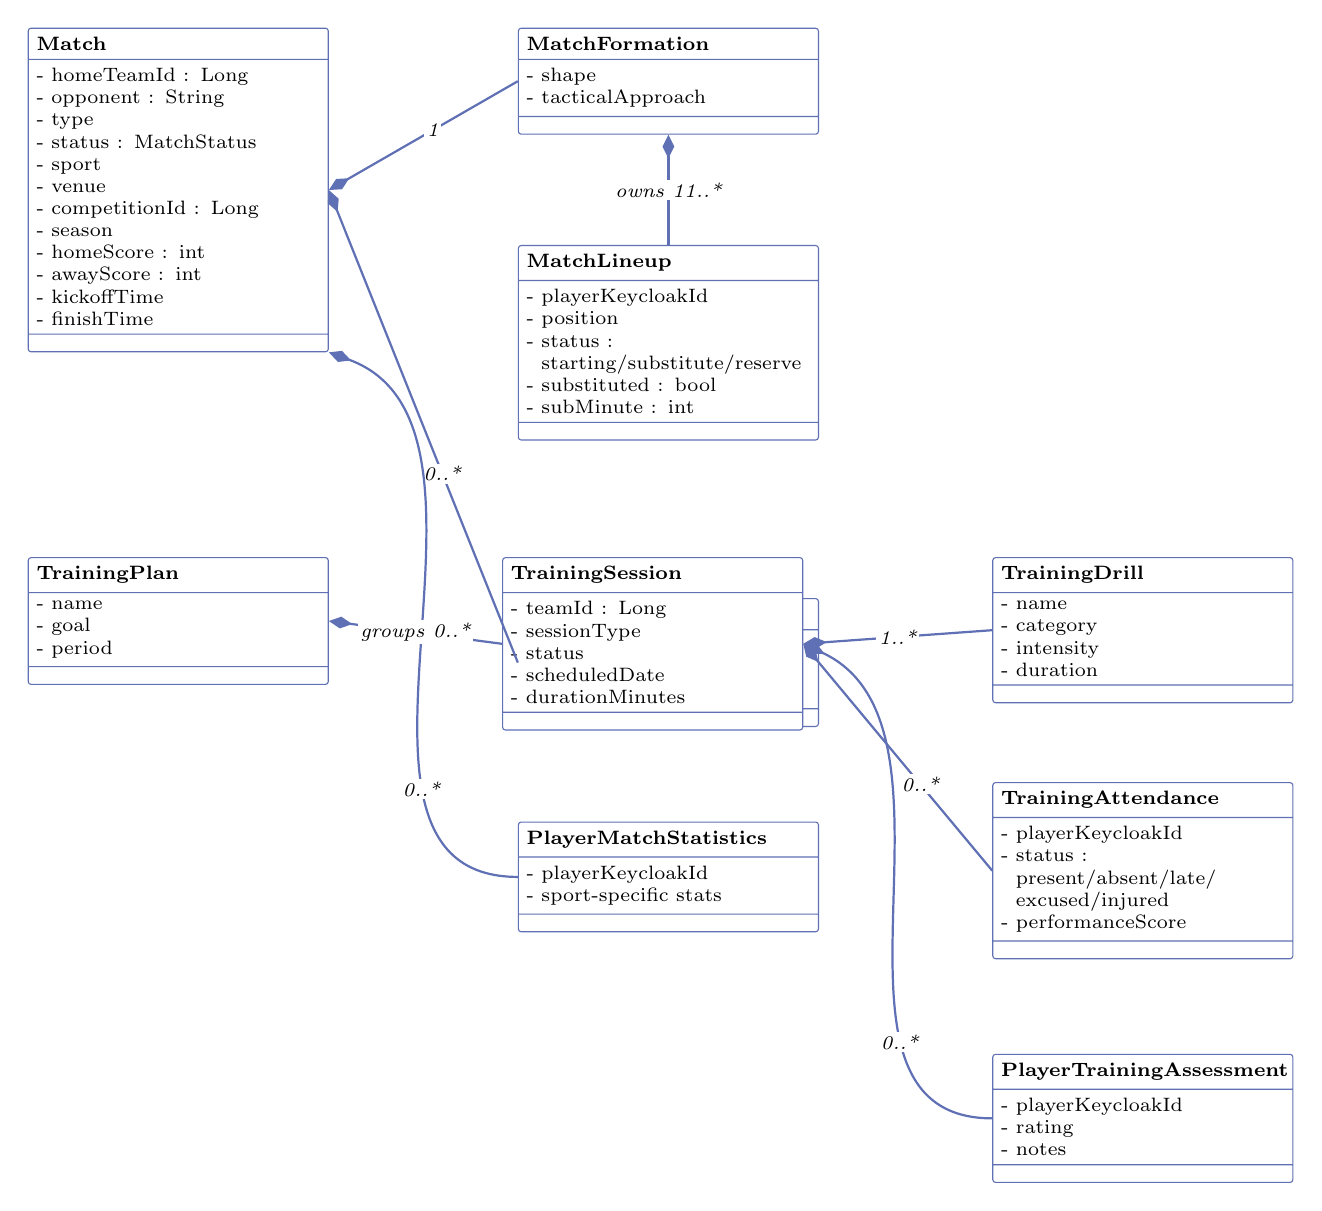
\begin{tikzpicture}[node distance=8mm,
   comp/.style={->,>={Stealth[length=2.4mm,open]},draw=dLine,thick}]

  %====================== MATCH SIDE ======================
  \UmlClass{match}{Match}{%
    - homeTeamId : Long\\
    - opponent : String\\
    - type\\
    - status : MatchStatus\\
    - sport\\
    - venue\\
    - competitionId : Long\\
    - season\\
    - homeScore : int\\
    - awayScore : int\\
    - kickoffTime\\
    - finishTime}{}

  \UmlClass[right=24mm of match.north east,anchor=north west]{form}{MatchFormation}{%
    - shape\\
    - tacticalApproach}{}

  \UmlClass[below=14mm of form]{line}{MatchLineup}{%
    - playerKeycloakId\\
    - position\\
    - status :\\
    \ \ starting/substitute/reserve\\
    - substituted : bool\\
    - subMinute : int}{}

  \UmlClass[below=20mm of line]{event}{MatchEvent}{%
    - type : EventType\\
    - minute : int\\
    - stoppage : int}{}

  \UmlClass[below=12mm of event]{stat}{PlayerMatchStatistics}{%
    - playerKeycloakId\\
    - sport-specific stats}{}

  %====================== TRAINING SIDE ======================
  \UmlClass[below=26mm of match.south west,anchor=north west]{plan}{TrainingPlan}{%
    - name\\
    - goal\\
    - period}{}

  \UmlClass[right=22mm of plan.north east,anchor=north west]{sess}{TrainingSession}{%
    - teamId : Long\\
    - sessionType\\
    - status\\
    - scheduledDate\\
    - durationMinutes}{}

  \UmlClass[right=24mm of sess.north east,anchor=north west]{drill}{TrainingDrill}{%
    - name\\
    - category\\
    - intensity\\
    - duration}{}

  \UmlClass[below=10mm of drill]{att}{TrainingAttendance}{%
    - playerKeycloakId\\
    - status :\\
    \ \ present/absent/late/\\
    \ \ excused/injured\\
    - performanceScore}{}

  \UmlClass[below=12mm of att]{assess}{PlayerTrainingAssessment}{%
    - playerKeycloakId\\
    - rating\\
    - notes}{}

  %====================== COMPOSITIONS ======================
  % filled diamond at the OWNER (whole) end = UML composition
  \tikzset{comp/.style={{Diamond[length=3mm]}-,draw=dLine,thick}}

  % Match owns formation, events, statistics
  \draw[comp] (match.east) -- node[lbl,pos=0.55]{\itshape 1} (form.west);
  \draw[comp] (match.east) -- node[lbl,pos=0.6]{\itshape 0..*} (event.west);
  \draw[comp] (match.south east) to[out=-20,in=180] node[lbl,pos=0.72]{\itshape 0..*} (stat.west);

  % Formation OWNS the starting XI (atomic match+formation+lineup)
  \draw[comp] (form.south) -- node[lbl,pos=0.5]{\itshape owns 11..*} (line.north);

  % TrainingPlan groups sessions; TrainingSession owns its children
  \draw[comp] (plan.east) -- node[lbl,pos=0.5]{\itshape groups 0..*} (sess.west);
  \draw[comp] (sess.east) -- node[lbl,pos=0.5]{\itshape 1..*} (drill.west);
  \draw[comp] (sess.east) -- node[lbl,pos=0.62]{\itshape 0..*} (att.west);
  \draw[comp] (sess.east) to[out=-25,in=180] node[lbl,pos=0.72]{\itshape 0..*} (assess.west);

\end{tikzpicture}%
}

\end{document}
